
\chapter{Introduction}

The theory we are going to study is a \textit{geometric theory}:

\textbf{Euclid's 5 Postulates:}
\begin{enumerate}
    \item For any two points $A$ and $B$, there is exactly one line that passes through them.
    \item Every line can be extended indefinitely in both directions.
    \item Given a point $O$ and a radius $R$, there exists exactly one circle centered at $O$ with radius $R$.
    \item All right angles are congruent.
    \item Given a line $R$ and a point $P$ not on $R$, there exists exactly one line through $P$ that is parallel to $R$.
\end{enumerate}

The fifth postulate is more complex than the others; over time, mathematicians tried several times to prove the fifth postulate based on the other four. It was later discovered that the fifth is independent of the others.

\textbf{Consequences:}
\begin{enumerate}
    \item There is no line parallel to $R$ through $P$ \\
    \quad $\rightarrow$ Planar elliptic geometries $[S^2]$
    \item There exist two or more lines parallel to $R$ through $P$ \\
    \quad $\rightarrow$ Planar hyperbolic geometries $[H^2]$
\end{enumerate}

\begin{figure}[H]
    \centering
    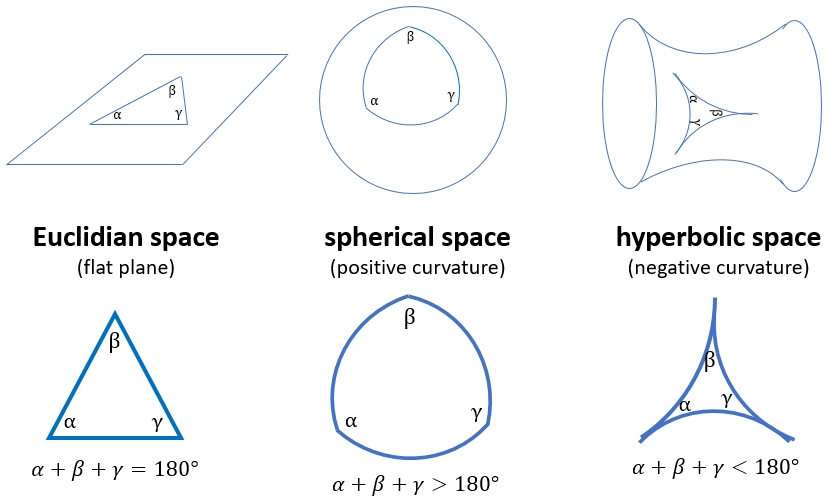
\includegraphics[width=0.5\textwidth]{assets/geometries.png}
    \caption{Elliptic and hyperbolic geometries}
\end{figure}

\subsubsection{Elliptic Geometry}

Planar elliptic geometry is a form of non-Euclidean geometry that rejects Euclid’s fifth postulate, which in Euclidean geometry guarantees the existence of exactly one parallel line through a given point. In elliptic geometry, no parallel lines exist; instead, every pair of lines eventually intersects.

A classic example of this is spherical geometry, where the “lines” are represented by great circles on a sphere.

\begin{figure}[H]
    \centering
    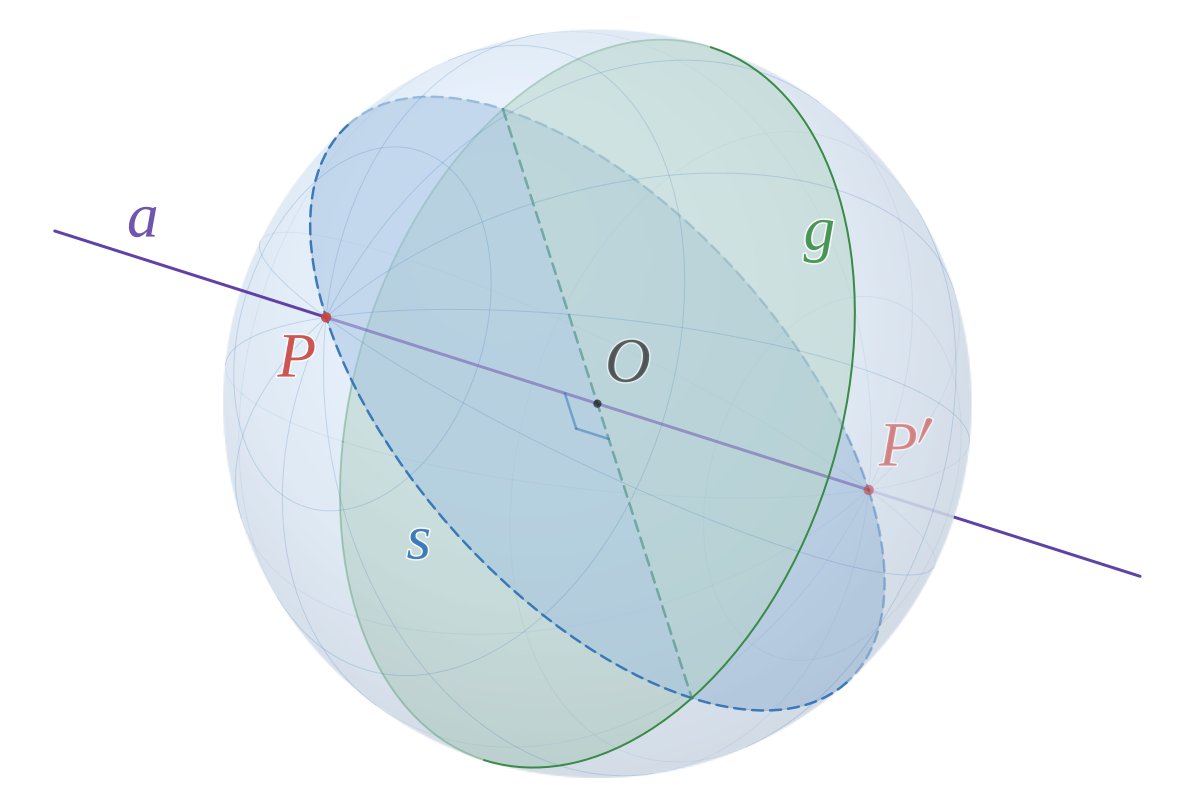
\includegraphics[width=0.5\textwidth]{assets/spherical_geometry.png}
    \caption{Spherical geometry}
\end{figure}

In this context, triangles, known as \textit{spherical triangles}, display an intriguing property: the sum of their interior angles exceeds 180° (a phenomenon known as spherical excess), with the excess being proportional to the area of the triangle.

\begin{figure}[H]
    \centering
    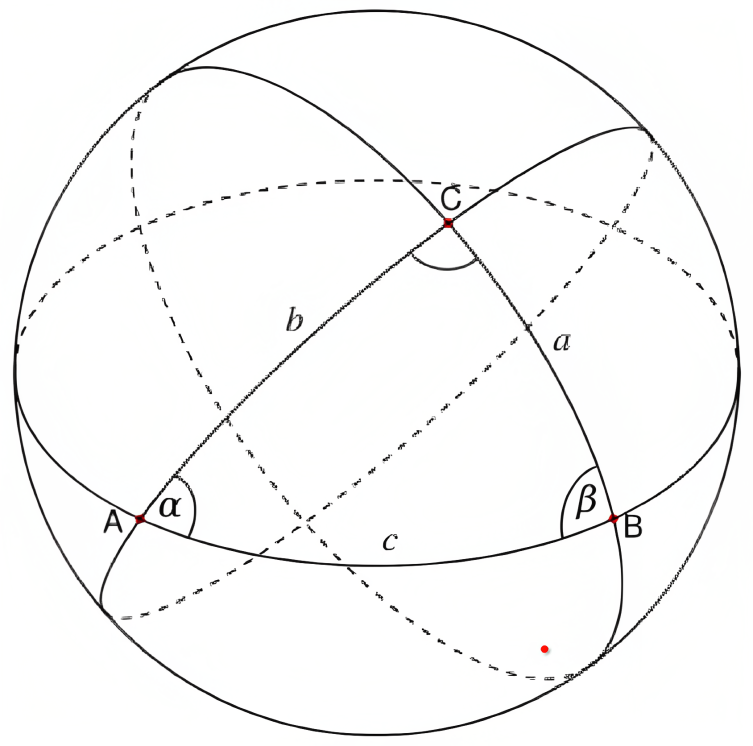
\includegraphics[width=0.5\textwidth]{assets/spherical_triangle.png}
    \caption{Spherical triangle}
\end{figure}

\subsubsection{Hyperbolic Geometry}

Planar hyperbolic geometry is a form of non-Euclidean geometry that rejects Euclid’s fifth postulate, which in Euclidean geometry guarantees the existence of exactly one parallel line through a given point. In hyperbolic geometry, multiple parallel lines exist, and the sum of the angles in a triangle is always less than 180°.

% \begin{figure}[H]
%     \centering
%     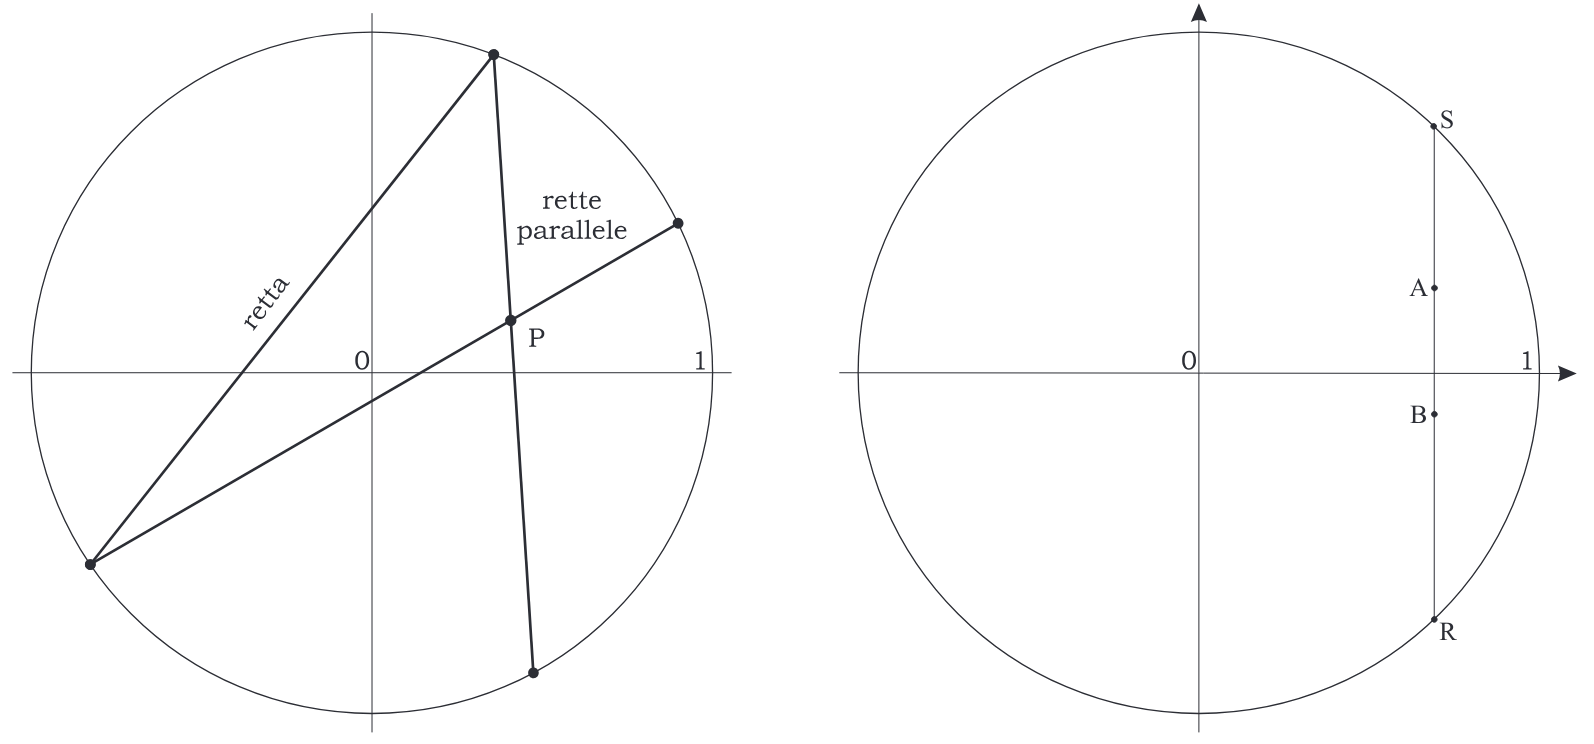
\includegraphics[width=0.5\textwidth]{assets/hyperbolic_geometry.png}
%     \caption{Hyperbolic geometry}
% \end{figure}

In this context, triangles—known as hyperbolic triangles—display an intriguing property: the sum of their interior angles is less than 180°, with the deficit being proportional to the area of the triangle.

\begin{figure}[H]
    \centering
    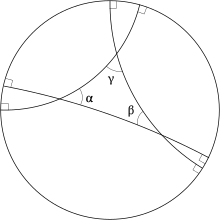
\includegraphics[width=0.5\textwidth]{assets/hyperbolic_triangle.png}
    \caption{Hyperbolic triangle}
\end{figure}

\subsubsection{Curva piana}


